% !TEX encoding = UTF-8 Unicode
% !TEX TS-program = xelatex
\begin{QUESTIONS}
    \begin{QUESTION}
        \begin{ExamInfo}{92}{學測}{單選}{1}
        \end{ExamInfo}
        \begin{ExamAnsRateInfo}{46}{74}{46}{18}
        \end{ExamAnsRateInfo}
        \begin{QBODY}
            試問有多少個正整數 $n$ 使得 $ \dfrac{1}{n} + \dfrac{2}{n} + \cdots + \dfrac{10}{n}$ 為整數? 
            \begin{QOPS} 
                \QOP $1$ 個 
                \QOP $2$ 個  
                \QOP $3$ 個 
                \QOP $4$ 個 
                \QOP $5$ 個
            \end{QOPS}
        \end{QBODY}
        \begin{QFROMS}
        \end{QFROMS}
        \begin{QTAGS}\QTAG{B2C1數列級數}\QTAG{B2C1-2級數}\end{QTAGS}
        \begin{QANS}
            (4)
        \end{QANS}
        \begin{QSOLLIST}
        \end{QSOLLIST}
        \begin{QEMPTYSPACE}
        \end{QEMPTYSPACE}
    \end{QUESTION}
    \begin{QUESTION}
        \begin{ExamInfo}{92}{學測}{單選}{2}
        \end{ExamInfo}
        \begin{ExamAnsRateInfo}{46}{83}{44}{11}
        \end{ExamAnsRateInfo}
        \begin{QBODY}
            若 $f(x)=x^3 - 2x^2 -x +5$,則多項式 $g(x)=f(f(x))$ 除以$(x-2)$ 所得的餘式為 
            \begin{QOPS} 
                \QOP $3 $
                \QOP $5 $
                \QOP $7 $
                \QOP $9 $
                \QOP $11$
            \end{QOPS}
        \end{QBODY}
        \begin{QFROMS}
        \end{QFROMS}
        \begin{QTAGS}\QTAG{B1C2多項式函數}\QTAG{B1C2-2多項式的運算與應用}\QTAG{餘式定理}\end{QTAGS}
        \begin{QANS}
            (5)
        \end{QANS}
        \begin{QSOLLIST}
        \end{QSOLLIST}
        \begin{QEMPTYSPACE}
        \end{QEMPTYSPACE}
    \end{QUESTION}
    \begin{QUESTION}
        \begin{ExamInfo}{92}{學測}{單選}{3}
        \end{ExamInfo}
        \begin{ExamAnsRateInfo}{41}{66}{36}{21}
        \end{ExamAnsRateInfo}
        \begin{QBODY}
            若 $(4 + 3i)(\cos \theta + i \sin \theta )$ 為小於 0 的實數, 則 $\theta$ 是第幾象限角? 
            \begin{QOPS} 
                \QOP 第一象限角 
                \QOP 第二象限角 
                \QOP 第三象限角 
                \QOP 第四象限角 
                \QOP 條件不足,無法判斷
            \end{QOPS}
        \end{QBODY}
        \begin{QFROMS}
        \end{QFROMS}
        \begin{QTAGS}\QTAG{B5C2三角函數II}\end{QTAGS}
        \begin{QANS}
            (2)
        \end{QANS}
        \begin{QSOLLIST}
        \end{QSOLLIST}
        \begin{QEMPTYSPACE}
        \end{QEMPTYSPACE}
    \end{QUESTION}
    \begin{QUESTION}
        \begin{ExamInfo}{92}{學測}{單選}{4}
        \end{ExamInfo}
        \begin{ExamAnsRateInfo}{49}{69}{47}{31}
        \end{ExamAnsRateInfo}
        \begin{QBODY}
            設 $ABC$ 為坐標平面上一三角形,$P$ 為平面上一點且 $\lvec{AP} = \dfrac{1}{5} \lvec{AB} + \dfrac{2}{5} \lvec{AC}$ , 則 $\dfrac{\triangle ABP \mbox{面積}}{ \triangle ABC \mbox{面積}}$等於 
            \begin{QOPS}
                \QOP $\dfrac{1}{5}$ 
                \QOP $\dfrac{1}{4}$ 
                \QOP $\dfrac{2}{5}$ 
                \QOP $\dfrac{1}{2}$         
                \QOP $\dfrac{2}{3}$
            \end{QOPS}
        \end{QBODY}
        \begin{QFROMS}
        \end{QFROMS}
        \begin{QTAGS}\QTAG{面積}\QTAG{B3C3-3面積與二階行列式}\QTAG{B3C3-1平面向量的表示法}\QTAG{B3C3平面向量}\QTAG{線性組合}\end{QTAGS}
        \begin{QANS}
            (3)
        \end{QANS}
        \begin{QSOLLIST}
        \end{QSOLLIST}
        \begin{QEMPTYSPACE}
        \end{QEMPTYSPACE}
    \end{QUESTION}
    \begin{QUESTION}
        \begin{ExamInfo}{92}{學測}{單選}{5}
        \end{ExamInfo}
        \begin{ExamAnsRateInfo}{22}{43}{15}{8}
        \end{ExamAnsRateInfo}
        \begin{QBODY}
            根據統計資料,在  $A$ 小鎮當某件訊息發布後, 
            $t$ 小時之內聽到該訊息的人口是全鎮人口的 $100(1- 2^{-kt})\%$ ,
            其中 $k$ 是某個大於 $0$ 的常數。
            今有某訊息,假設在發布後 $3$ 小時之內已經有 $70\%$ 的人口聽到該訊息。
            又設最快要 $T$ 小時後,有 $99\%$ 的人口已聽到該訊息,則 $T$ 最接近下列哪一個選項?
            \begin{QOPS} 
                \QOP $5$小時        
                \QOP $7\frac{1}{2}$小時
                \QOP $9$小時 
                \QOP $11\frac{1}{2}$小時 
                \QOP $13$小時
            \end{QOPS}
        \end{QBODY}
        \begin{QFROMS}
        \end{QFROMS}
        \begin{QTAGS}\QTAG{應用問題}\QTAG{B1C3指對數函數}\QTAG{B1C3-5指數與對數的應用}\end{QTAGS}
        \begin{QANS}
            (4)
        \end{QANS}
        \begin{QSOLLIST}
        \end{QSOLLIST}
        \begin{QEMPTYSPACE}
        \end{QEMPTYSPACE}
    \end{QUESTION}
\end{QUESTIONS}
\begin{QUESTIONS}
    \begin{QUESTION}
        \begin{ExamInfo}{92}{學測}{多選}{6}
        \end{ExamInfo}
        \begin{ExamAnsRateInfo}{41}{71}{40}{12}
        \end{ExamAnsRateInfo}
        \begin{QBODY}
            如右圖,兩直線 $L_1$ 、 $L_2$ 之方程式分別為 $L_1 : x+ay+b=0$, $L_2 :x+cy+d=0$;試問下列哪些選項是正確的? 
            \begin{QOPS} 
                \QOP $a>0$ 
                \QOP $b>0$ 
                \QOP $c>0$ 
                \QOP $d>0$ 
                \QOP $a<c$ 
            \end{QOPS}
            
            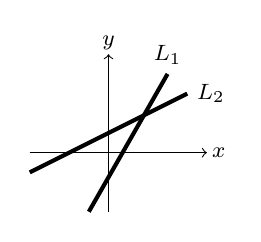
\begin{tikzpicture}[scale=.5]\footnotesize
            \begin{scope}
            \pgfsetarrowsend{latex}
            \draw[->]  (-2,0) to(2.5,0);
            \draw[->] (0,-1.5) to (0,2.5);
            \end{scope}
            \pgfsetlinewidth{1.5pt}
            \node at (0,2.8) {$y$};
            \node at (2.8,0) {$x$};
            \draw (-2,-0.5) to (2,1.5) node[right] {$L_2$};
            \draw (-.5,-1.5) to (1.5,2)node[above] {$L_1$} ;
            \end{tikzpicture}
        \end{QBODY}
        \begin{QFROMS}
        \end{QFROMS}
        \begin{QTAGS}\QTAG{B3C2-1直線方程式及其圖形}\QTAG{圖形}\QTAG{B3C2直線與圓}\end{QTAGS}
        \begin{QANS}
            (4)(5)
        \end{QANS}
        \begin{QSOLLIST}
        \end{QSOLLIST}
        \begin{QEMPTYSPACE}
        \end{QEMPTYSPACE}
    \end{QUESTION}
    \begin{QUESTION}
        \begin{ExamInfo}{92}{學測}{多選}{7}
        \end{ExamInfo}
        \begin{ExamAnsRateInfo}{45}{79}{41}{15}
        \end{ExamAnsRateInfo}
        \begin{QBODY}
            如右圖,$ABCD-EFGH$ 為一平行六面體,$J$ 為四邊形 $BCGF$ 的中心,
            如果 $\lvec{AJ} = a \lvec{AB} + b\lvec{AD}+ c\lvec{AE}$,
            試問下列哪些選項是正確的? 
            \begin{QOPS} 
                \QOP $\frac{1}{3} < b < \frac{2}{3}$ 
                \QOP $a + b + c = 2$  
                \QOP $a=1$
                \QOP $a=2c$ 
                \QOP $a=b$
            \end{QOPS}
        
            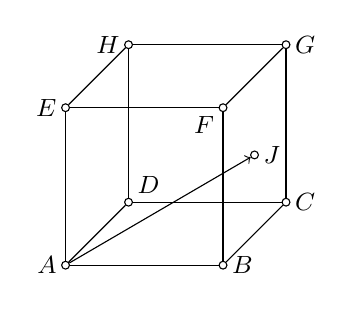
\begin{tikzpicture}
                \begin{scope}
                \small
                \tikzstyle{vnode}=[draw,circle,inner sep =1pt];
                \node[vnode] (v000) at (0,0) {};
                \node[anchor =south west] (t000) at (v000) {$D$};
                \node[vnode] (v001) at (0,2) {$$};
                \node[anchor =east] (t000) at (v001) {$H$};
                \node[vnode] (v011) at (2,2) {$$};
                \node[anchor =west] (t011) at (v011) {$G$};
                \node[vnode] (v010) at (2,0) {$$};
                \node[anchor =west] (t010) at (v010) {$C$};
                \node[vnode] (v100) at (-.8,-.8) {$$};
                \node[anchor =east] (t100) at (v100) {$A$};
                \node[vnode] (v101) at (-.8,1.2) {$$};
                \node[anchor =east] (t101) at (v101) {$E$};
                \node[vnode] (v111) at (1.2,1.2) {$$};
                \node[anchor =north east] (t111) at (v111) {$F$};
                \node[vnode] (v110) at (1.2,-0.8) {$$};
                \node[anchor =west] (t110) at (v110) {$B$};
                \node[vnode] (vJ) at (1.6, .6) {$$};
                \node[anchor =west] (tJ) at (vJ) {$J$};
                \foreach \i in {01,10,11}{
                    \draw (v0\i) to (v1\i);
                    \draw (v\i  0) to (v\i 1);
                }
                \draw (v000) to[dashed] (v100);
                \draw (v000) to[dashed] (v010);
                \draw (v000) to[dashed] (v001);
                \draw (v001) to (v011);
                \draw (v100) to (v110);
                \draw (v101) to (v111);
                \draw[->] (v100) to (vJ);
                \end{scope}
            \end{tikzpicture}
        \end{QBODY}
        \begin{QFROMS}
        \end{QFROMS}
        \begin{QTAGS}\QTAG{B4C1-2空間向量的坐標表示法}\QTAG{B4C1空間向量}\end{QTAGS}
        \begin{QANS}
            (1)(2)(3)(4)
        \end{QANS}
        \begin{QSOLLIST}
        \end{QSOLLIST}
        \begin{QEMPTYSPACE}
        \end{QEMPTYSPACE}
    \end{QUESTION}
    \begin{QUESTION}
        \begin{ExamInfo}{92}{學測}{多選}{8}
        \end{ExamInfo}
        \begin{ExamAnsRateInfo}{55}{86}{60}{19}
        \end{ExamAnsRateInfo}
        \begin{QBODY}
            以下各數何者為正? 
            \begin{QOPS} 
                \QOP $\sqrt{2} - \sqrt[3]{2}$ 
                \QOP $\log_{2} 3-1$ 
                \QOP $\log_{3}2 -1$ 
                \QOP $\log_{\frac{1}{2}} 3$ 
                \QOP $\log_{\frac{1}{3}} \frac{1}{2}$ 
            \end{QOPS}
        \end{QBODY}
        \begin{QFROMS}
        \end{QFROMS}
        \begin{QTAGS}\QTAG{B1C3-2指數函數}\QTAG{B1C3指對數函數}\QTAG{指數律}\end{QTAGS}
        \begin{QANS}
            (1)(2)(5)
        \end{QANS}
        \begin{QSOLLIST}
        \end{QSOLLIST}
        \begin{QEMPTYSPACE}
        \end{QEMPTYSPACE}
    \end{QUESTION}
    \begin{QUESTION}
        \begin{ExamInfo}{92}{學測}{多選}{9}
        \end{ExamInfo}
        \begin{ExamAnsRateInfo}{24}{42}{19}{11}
        \end{ExamAnsRateInfo}
        \begin{QBODY}
            下列哪些函數的最小正週期為 $\pi$ ? 
            \begin{QOPS} 
                \QOP $\sin x + \cos x$ 
                \QOP $\sin x - \cos x$ 
                \QOP $|\sin x + \cos x|$
                \QOP $|\sin x - \cos x|$ 
                \QOP $|\sin x| + |\cos x|$
            \end{QOPS}
        \end{QBODY}
        \begin{QFROMS}
        \end{QFROMS}
        \begin{QTAGS}\QTAG{B5C2-1一般三角函數的性質與圖形}\QTAG{B5C2三角函數II}\end{QTAGS}
        \begin{QANS}
            (3)(4)
        \end{QANS}
        \begin{QSOLLIST}
        \end{QSOLLIST}
        \begin{QEMPTYSPACE}
        \end{QEMPTYSPACE}
    \end{QUESTION}
    \begin{QUESTION}
        \begin{ExamInfo}{92}{學測}{多選}{10}
        \end{ExamInfo}
        \begin{ExamAnsRateInfo}{21}{43}{14}{6}
        \end{ExamAnsRateInfo}
        \begin{QBODY}
            假設坐標平面上一非空集合 $S$ 試問下列哪些敘述對 $S$ 內的點 $(x, y)$ 具有以下性質:「若  $x > 0$,則 $y > 0$」。 試問下列哪些敘述對 $S$ 內的點 $(x, y)$ 必定成立? 
            \begin{QOPS} 
                \QOP 若 $x \leq 0$,則 $y \leq 0$ ;
                \QOP 若 $y \leq 0$, 則 $x \leq 0$;
                \QOP 若 $y \leq 0$,則 $x \leq 0$ ; 
                \QOP 若 $x >1$,則 $y>0$;  \QOP 若 $y<0$ ,則 $x \leq 0$。
            \end{QOPS}
        \end{QBODY}
        \begin{QFROMS}
        \end{QFROMS}
        \begin{QTAGS}\QTAG{不是99課綱}\end{QTAGS}
        \begin{QANS}
            (2)(4)(5)
        \end{QANS}
        \begin{QSOLLIST}
        \end{QSOLLIST}
        \begin{QEMPTYSPACE}
        \end{QEMPTYSPACE}
    \end{QUESTION}
    \begin{QUESTION}
        \begin{ExamInfo}{92}{學測}{多選}{11}
        \end{ExamInfo}
        \begin{ExamAnsRateInfo}{24}{43}{18}{11}
        \end{ExamAnsRateInfo}
        \begin{QBODY}
            設 $\pi_a : x-4y +az=10$ ($a$為常數), $E_1 :x-2y+z=5$ 及 $E_2  :2x-5y+4z=3$ 為坐標空間中的三個平面。
            試問下列哪些敘述是正確的?
            
            \begin{QOPS} 
                \QOP 存在實數 $a$ 使得 $\pi_a$ 與 $E_1$ 平行;
                \QOP 存在實數 $a$ 使得 $\pi_a$ 與 $E_1$ 垂直;
                \QOP 存在實數 $a$ 使得 $\pi_a$ , $E_1$, $E_2$ 交於一點; 
                \QOP 存在實數 $a$ 使得 $\pi_a, E_1, E_2 $ 交於一直線;
                \QOP 存在實數 $a$ 使得 $\pi_a$, $E_1$ , $E_2$ 沒有共同交點。\end{QOPS}
        \end{QBODY}
        \begin{QFROMS}
        \end{QFROMS}
        \begin{QTAGS}\QTAG{B4C3矩陣}\QTAG{B4C3-1線性方程組與矩陣}\QTAG{方程組}\end{QTAGS}
        \begin{QANS}
            (2)(3)(5)
        \end{QANS}
        \begin{QSOLLIST}
        \end{QSOLLIST}
        \begin{QEMPTYSPACE}
        \end{QEMPTYSPACE}
    \end{QUESTION}
\end{QUESTIONS}
\begin{QUESTIONS}
    \begin{QUESTION}
        \begin{ExamInfo}{92}{學測}{填充}{A}
        \end{ExamInfo}
        \begin{ExamAnsRateInfo}{37}{74}{31}{6}
        \end{ExamAnsRateInfo}
        \begin{QBODY}
            設 $a_1,a_2,\cdots,a_{50}$ 是從 $-1,0,1$ 這三個整數中取值的數列。若 $a_1 +a_2 + \cdots + a_{50} = 9$ 且 $(a_1+1)^2 +(a_2 +1)^2 + \cdots + (a_{50} +1)^2 =107$, 則 $a_1,a_2,\cdots,a_{50}$ 當中有幾項是 $0$?答: 
            $\TCNBOX{\TCN\TCN}$ 項。
        \end{QBODY}
        \begin{QFROMS}
        \end{QFROMS}
        \begin{QTAGS}\QTAG{B2C1數列級數}\QTAG{特殊數列}\QTAG{B2C1-2級數}\QTAG{B2C1-1數列}\end{QTAGS}
        \begin{QANS}
            $11$
        \end{QANS}
        \begin{QSOLLIST}
        \end{QSOLLIST}
        \begin{QEMPTYSPACE}
        \end{QEMPTYSPACE}
    \end{QUESTION}
    \begin{QUESTION}
        \begin{ExamInfo}{92}{學測}{填充}{B}
        \end{ExamInfo}
        \begin{ExamAnsRateInfo}{64}{93}{70}{29}
        \end{ExamAnsRateInfo}
        \begin{QBODY}
            金先生在提款時忘了帳號密碼,但他還記得密碼的四位數字中,有兩個 $3$, 一個 $8$,一個 $9$,於是他就用這四個數字隨意排成一個四位數輸入提款機嘗試。請問他只試一次就成功的機率有多少? $\TCNBOX{\FR{\TCN}{\TCN\TCN}}$
        \end{QBODY}
        \begin{QFROMS}
        \end{QFROMS}
        \begin{QTAGS}\QTAG{B2C3機率}\QTAG{B2C3-2機率的定義與性質}\end{QTAGS}
        \begin{QANS}
            $\frac{1}{12}$
        \end{QANS}
        \begin{QSOLLIST}
        \end{QSOLLIST}
        \begin{QEMPTYSPACE}
        \end{QEMPTYSPACE}
    \end{QUESTION}
    \begin{QUESTION}
        \begin{ExamInfo}{92}{學測}{填充}{C}
        \end{ExamInfo}
        \begin{ExamAnsRateInfo}{27}{52}{21}{8}
        \end{ExamAnsRateInfo}
        \begin{QBODY}
            設 $A(1,0)$ 與 $B(b,0)$ 為坐標平面上的兩點, 其中 $b>1$。 
            若拋物線 $\Gamma : y^2=4x$ 上有一點 $P$ 使得 $\triangle ABP$ 為一正三角形,則 $b= 
            \TCNBOX{\TCN}$。
        \end{QBODY}
        \begin{QFROMS}
        \end{QFROMS}
        \begin{QTAGS}\QTAG{B4C4二次曲線}\QTAG{B4C4-1拋物線}\QTAG{圖形}\end{QTAGS}
        \begin{QANS}
            $5$
        \end{QANS}
        \begin{QSOLLIST}
        \end{QSOLLIST}
        \begin{QEMPTYSPACE}
        \end{QEMPTYSPACE}
    \end{QUESTION}
    \begin{QUESTION}
        \begin{ExamInfo}{92}{學測}{填充}{D}
        \end{ExamInfo}
        \begin{ExamAnsRateInfo}{16}{39}{7}{2}
        \end{ExamAnsRateInfo}
        \begin{QBODY}
            設 $P$ 為雙曲線 $\dfrac{x^2}{9} - \dfrac{y^2}{16} = 1$ 上的一點且位在第一象限。若 $F_1$,  $F_2$ 為此雙曲線的兩個焦點,且 $\overline{PF}_1 : \overline{PF}_2 = 1:3 $,則 $\triangle F_1PF_2$ 的周長等於 $
            \TCNBOX{\TCN\TCN}$。
        \end{QBODY}
        \begin{QFROMS}
        \end{QFROMS}
        \begin{QTAGS}\QTAG{B4C4-3雙曲線}\QTAG{B4C4二次曲線}\QTAG{圖形}\end{QTAGS}
        \begin{QANS}
            $22$
        \end{QANS}
        \begin{QSOLLIST}
        \end{QSOLLIST}
        \begin{QEMPTYSPACE}
        \end{QEMPTYSPACE}
    \end{QUESTION}
    \begin{QUESTION}
        \begin{ExamInfo}{92}{學測}{填充}{E}
        \end{ExamInfo}
        \begin{ExamAnsRateInfo}{21}{37}{17}{9}
        \end{ExamAnsRateInfo}
        \begin{QBODY}
            在坐標空間中,通過 $O(0,0,0)$, $N(0,0,1)$, $P(\dfrac{1}{4}, \dfrac{\sqrt{11}}{4}, -\dfrac{1}{2})$ 三點的平面與球面  $S: x^2+y^2+z^2=1$相交於一個圓 $C$,則圓 $C$ 的劣弧 $NP$ 的弧長等於 
            $\TCNBOX{\FR{\TCN}{\TCN} \pi} $。
        \end{QBODY}
        \begin{QFROMS}
        \end{QFROMS}
        \begin{QTAGS}\QTAG{不是99課綱}\end{QTAGS}
        \begin{QANS}
            $\frac{2}{3}\pi$
        \end{QANS}
        \begin{QSOLLIST}
        \end{QSOLLIST}
        \begin{QEMPTYSPACE}
        \end{QEMPTYSPACE}
    \end{QUESTION}
    \begin{QUESTION}
        \begin{ExamInfo}{92}{學測}{填充}{F}
        \end{ExamInfo}
        \begin{ExamAnsRateInfo}{35}{67}{31}{7}
        \end{ExamAnsRateInfo}
        \begin{QBODY}
            設 $k$ 為一整數,若方程式 $kx^2 + 7x +1= 0$ 有兩個相異實根,且兩根的乘積介於 $\dfrac{5}{71}$ 與 $\dfrac{6}{71}$之間,則 $k=\TCNBOX{\TCN\TCN}$。
        \end{QBODY}
        \begin{QFROMS}
        \end{QFROMS}
        \begin{QTAGS}\QTAG{B1C2-3多項式方程式}\QTAG{根與係數的關係}\QTAG{B1C2多項式函數}\QTAG{韋達定理}\end{QTAGS}
        \begin{QANS}
            $12$
        \end{QANS}
        \begin{QSOLLIST}
        \end{QSOLLIST}
        \begin{QEMPTYSPACE}
        \end{QEMPTYSPACE}
    \end{QUESTION}
    \begin{QUESTION}
        \begin{ExamInfo}{92}{學測}{填充}{G}
        \end{ExamInfo}
        \begin{ExamAnsRateInfo}{15}{41}{4}{0}
        \end{ExamAnsRateInfo}
        \begin{QBODY}
            在只有皮尺沒有梯子的情形下,想要測出一拋物線形拱門的高度。
            已知此拋物線以過最高點的鉛垂線為對稱軸。
            現甲、乙兩人以皮尺測得拱門底部寬為 $6$ 公尺,且距底部 $\frac{3}{2}$ 公尺高處其寬為 $5$ 公尺。
            利用這些數據可推算出拱門的高度為$\TCNBOX{\FR{\TCN\TCN}{\TCN\TCN}}$ 公尺。
        \end{QBODY}
        \begin{QFROMS}
        \end{QFROMS}
        \begin{QTAGS}\QTAG{B1C2多項式函數}\QTAG{圖形}\QTAG{二次多項式}\QTAG{B1C2-1簡單的多項式及圖形}\QTAG{最值}\end{QTAGS}
        \begin{QANS}
            $\dfrac{54}{11}$
        \end{QANS}
        \begin{QSOLLIST}
        \end{QSOLLIST}
        \begin{QEMPTYSPACE}
        \end{QEMPTYSPACE}
    \end{QUESTION}
    \begin{QUESTION}
        \begin{ExamInfo}{92}{學測}{填充}{H}
        \end{ExamInfo}
        \begin{ExamAnsRateInfo}{17}{36}{12}{3}
        \end{ExamAnsRateInfo}
        \begin{QBODY}
            某次數學測驗共有 $25$ 題單一選擇題,每題都有五個選項,每答對一題可得 $4$ 分,答錯倒扣 $1$ 分。某生確定其中 $16$ 題可答對;有 $6$ 題他確定五個選項中有兩個選項不正確,因此這 $6$ 題他就從剩下的選項中分別猜選一個;另外 $3$ 題只好亂猜,則他這次測驗得分之期望值為 
            \TCNBOX{\TCN\TCN} 分。(計算到整數為止,小數點以後四捨五入。)
        \end{QBODY}
        \begin{QFROMS}
        \end{QFROMS}
        \begin{QTAGS}\QTAG{B5C1機率與統計}\end{QTAGS}
        \begin{QANS}
            $68$
        \end{QANS}
        \begin{QSOLLIST}
        \end{QSOLLIST}
        \begin{QEMPTYSPACE}
        \end{QEMPTYSPACE}
    \end{QUESTION}
    \begin{QUESTION}
        \begin{ExamInfo}{92}{學測}{填充}{I}
        \end{ExamInfo}
        \begin{ExamAnsRateInfo}{38}{70}{35}{9}
        \end{ExamAnsRateInfo}
        \begin{QBODY}
            根據統計資料,$1$ 月份台北地區的平均氣溫是攝氏 $16$ 度,
            標準差是攝氏 $3.5$ 度。一般外國朋友比較習慣用華氏溫度來表示冷熱,
            已知當攝氏溫度為 $x$ 時,華氏溫度為 $y =\dfrac{9}{5}x + 32$;
            若用華氏溫度表示,則 1 月份台北地區的平均氣溫是華氏 
            \TCNBOX{\TCN\TCN.\TCN} 度,
            標準差是華氏 
            \TCNBOX{\TCN.\TCN} 度。(計算到小數點後第一位,以下四捨五入。)
        \end{QBODY}
        \begin{QFROMS}
        \end{QFROMS}
        \begin{QTAGS}\QTAG{平均數}\QTAG{B2C4-1一維數據分析}\QTAG{B2C4數據分析}\QTAG{線性公式}\QTAG{標準差}\end{QTAGS}
        \begin{QANS}
            $60.8$, $6.3$
        \end{QANS}
        \begin{QSOLLIST}
        \end{QSOLLIST}
        \begin{QEMPTYSPACE}
        \end{QEMPTYSPACE}
    \end{QUESTION}
\end{QUESTIONS}
